\documentclass{beamer}

\usetheme{default}

\usepackage{listings}
\usepackage{xcolor}
\usepackage[spanish]{babel}
\usepackage{graphicx}
\usepackage{fancyhdr}

\lstset{
  language=bash,
  basicstyle=\ttfamily\small,
  keywordstyle=\color{blue},
  commentstyle=\color{gray},
  stringstyle=\color{red},
  showstringspaces=false,
  tabsize=4,
  breaklines=true,
  breakatwhitespace=true
}

\setbeamertemplate{footline}{
  \begin{beamercolorbox}[sep=1em,ht=2.5ex,wd=\paperwidth]{footline}%
    \insertframenumber/\inserttotalframenumber \hspace{2em}  Diego Nieto \hspace{2em}  \raisebox{-0.3\height}{
\includegraphics[height=0.4cm]{fluendo-logo.png}}
  \end{beamercolorbox}
}

\title{Introducción a GStreamer}
\author{Diego Nieto Muñoz @ Fluendo}
\date{\today}

\begin{document}

\begin{frame}
  \titlepage
\end{frame}

\begin{frame}
  \frametitle{Quien soy?}
  \begin{itemize}
    \item Senior multimedia engineer at Fluendo
    \begin{itemize}
      \item Audio/Video codecs
      \item Digital microscopes
      \item Drones
    \end{itemize}
    \item Mirada PLC
    \begin{itemize}
      \item Native C++ with Qt Streaming player and FFmpeg
      \item Integration of Netflix, Disney+ as embedded applications
      \item Screencapture for videogames
    \end{itemize}
    \item BSC-CNS
    \begin{itemize}
      \item OpenCL and CUDA offloading algorithms
      \item OpenMP and MPI parallelizations
    \end{itemize}
    \item USC
    \item ULPGC
  \end{itemize}
\end{frame}

\begin{frame}
  \frametitle{Agenda}
  \begin{itemize}
    \item ¿Qué es GStreamer?
    \item ¿Quién lo usa?
    \item ¿Para qué lo podemos usar?
    \item Conceptos básicos de GStreamer y multimedia
    \item Cómo se hacen pipelines
    \item Cómo hacer nuestra primera aplicación
    \begin{itemize}
      \item C
      \item Python
    \end{itemize}
    \item Dónde buscar referencias
  \end{itemize}
\end{frame}

\begin{frame}{¿Que es GStreamer?}
\begin{itemize}
  \item Multimedia framework
  \item Based on plugins
  \item Data agnostic
  \item Multiplatform
\end{itemize}
\end{frame}

\begin{frame}{¿Quién lo usa?}
Big companies:
\begin{itemize}
  \item DELL
  \item HP
  \item IGEL
  \item Citrix
  \item HbbTV
\end{itemize}
Fluendo CS clients:
\begin{itemize}
  \item Partner Electronics
  \item Vicon
  \item ScoutDI
  \item Brightsign
  \item TZ Electronics
\end{itemize}
\end{frame}

\begin{frame}{¿Para qué lo podemos usar?}
Use cases:
\begin{itemize}
  \item Screencapture for videogames
  \item Microscopes
  \item Webcams
  \item Virtual environments
  \item Video streaming
  \item DVB TV
  \item ...
\end{itemize}
\end{frame}

\begin{frame}{GStreamer History}
\begin{itemize}
  \item GStreamer 0.1-0.9 - since 1999
  \item GStreamer 0.10 - December 2005
  \item GStreamer 1.0 - September 24, 2012
  \begin{itemize}
    \item HW dec/enc with GPU
    \item Dynamic pipelines
    \item Zero copy
    \item API enhancements
  \end{itemize}
\end{itemize}
\end{frame}

\begin{frame}{Conceptos básicos de GStreamer y multimedia I}
  \begin{itemize}
    \item video codecs: h265, h265, AV1
    \item audio codecs: AAC, MP3
    \item subtitles: closedcaptions, TTML
    \item images: jpeg, png
    \item containers: mp4, mpegts
    \item demuxers: qtdemux(mp4),tsdemux(ts)
    \item tcp streaming protocols: DASH, HLS
    \item udp protocols: udp, WebRTC
    \item formats: RGBA, YUV, NV12
    \item ...
  \end{itemize}
\end{frame}

\begin{frame}{Conceptos básicos de GStreamer y multimedia II}
  ¿Qué es YUV?
  \begin{itemize}
    \item Y (Luminancia): Esta componente lleva la información de brillo de la imagen y representa la escala de grises. Es decir, determina la intensidad luminosa de un píxel y define el contraste y la claridad de la imagen.
    \item U (Crominancia azul-diferencia): Esta componente representa la diferencia entre la luminancia y la componente azul (B) de la imagen. Lleva información sobre la cantidad de color azul en la imagen.
    \item V (Crominancia rojo-diferencia): Similar a la componente U, la componente V representa la diferencia entre la luminancia y la componente roja (R) de la imagen. Lleva información sobre la cantidad de color rojo en la imagen.
  \end{itemize}
  Compresión con pérdida de información no apreciable
\end{frame}

\begin{frame}{Conceptos básicos de GStreamer y multimedia III}
  \begin{figure}
    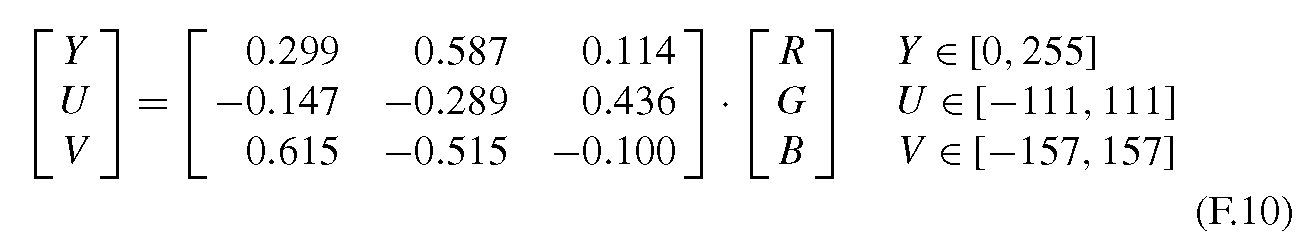
\includegraphics[width=1\textwidth]{rgba-to-yuv.png}
    \caption{YUV conversion}
  \end{figure}
\end{frame}

\begin{frame}{Conceptos básicos de GStreamer y multimedia IV}
  \begin{figure}
    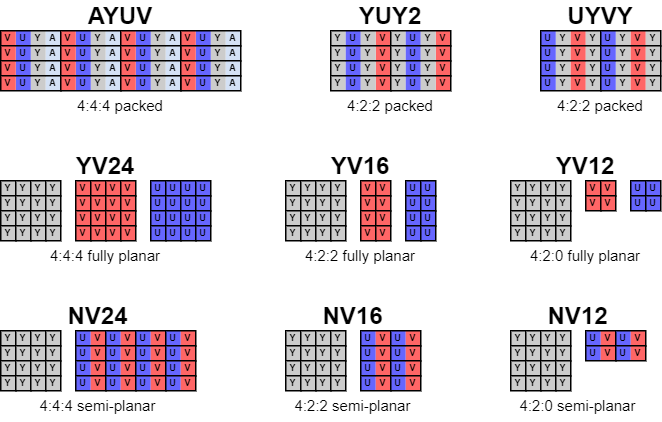
\includegraphics[width=1\textwidth]{formats.png}
    \caption{YUV compressed formats}
  \end{figure}
\end{frame}

\begin{frame}{GStreamer architecture}
  \begin{figure}
    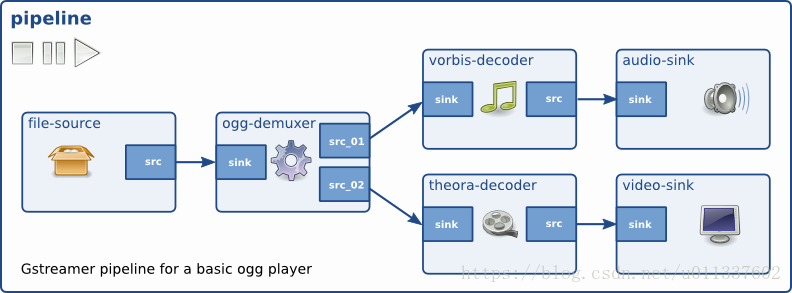
\includegraphics[width=1\textwidth]{gst-architecture.png}
    \caption{GStreamer architecture}
  \end{figure}
\end{frame}

\begin{frame}{GStreamer architecture - Elements}
\begin{itemize}
  \item The most important object in GStreamer for the application programmer
  \item An element is the basic building block for a media pipeline
  \item Normally an element has one specific function
  \item By chaining together several elements, you create a pipeline that can do a specific task, for example media playback or recording
  \item Can be visualized as black boxes - on the one end, you might put something in, the element does something with it and something else comes out at the other side.
\end{itemize}
\end{frame}

\begin{frame}{GStreamer architecture - Main elements}
\begin{itemize}
  \item Source elements generate data for use by a pipeline
  \item Source elements do not accept data, they only generate data
  \item Sink elements are end points in a media pipeline.
  \item They accept data but do not produce anything.
  \item Filters and filter-like elements (convertors, demuxers, muxers and encoders/decoders have both input and outputs pads)
\end{itemize}
\end{frame}

\begin{frame}{GStreamer architecture - Pads}
\begin{itemize}
  \item The pads are the element's interface to the outside world
  \item GStreamer defines two pad directions: source pads and sink pads
  \item Data streams from one element's source pad to another element's sink pad
  \item The specific type of media that the element can handle will be exposed by the pad's capabilities (caps)
\end{itemize}
\end{frame}

\begin{frame}{GStreamer architecture - Caps}
\begin{itemize}
  \item Caps - capabilities of a pad
  \item Describe the type of data that is streamed between two pads, or that one pad (template) supports
  \item Purposes:
    \begin{itemize}
      \item Autoplugging
      \item Compatibility detection
      \item Metadata
      \item Filtering
    \end{itemize}
\end{itemize}
\end{frame}

\begin{frame}{GStreamer architecture - Bins and pipelines}
\begin{itemize}
  \item A bin is a container for a collection of elements
  \item Bins are elements
  \item A pipeline is a top-level bin. It provides a bus for the application and manages the synchronization for its children
  \item (A bus is a simple system that takes care of forwarding messages from the streaming threads to an application in its own thread context.)
\end{itemize}
\end{frame}

\begin{frame}{GStreamer architecture - communication}
  \begin{figure}
    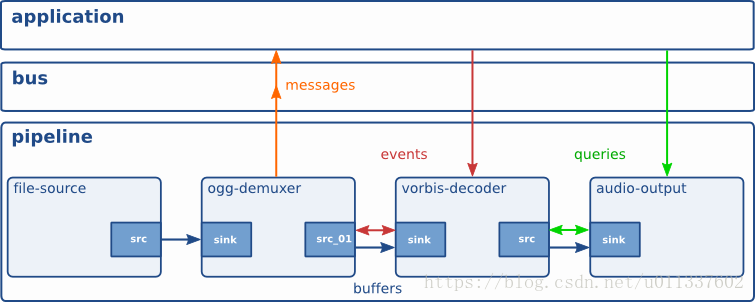
\includegraphics[width=1\textwidth]{gst-comm.png}
    \caption{GStreamer architecture}
  \end{figure}
\end{frame}

\begin{frame}{GStreamer architecture - communication}
\begin{itemize}
  \item Downstream and upstream communication
  \item Buffers - objects for passing streaming data between elements in the pipeline (downstream)
  \item Events - objects sent between elements or from the application to elements (downstream/upstream)
  \item Messages - objects posted by elements on the pipeline's message bus, where they will be held for collection by the application (eof, errors, tags, state changes, bufferingstate, redirects etc.)
  \item Queries - allow applications to request information such as duration or current playback position from the pipeline (downstream/upstream)
\end{itemize}
\end{frame}

\begin{frame}{GStreamer architecture - playback states}
  \begin{itemize}
    \item NULL: This is the initial state of an element.
    \item READY: The element should be prepared to go to PAUSED.
    \item PAUSED: The element should be ready to accept and process data. Sink elements, however, only accept one buffer and then block.
    \item PLAYING: The same as PAUSED except for live sources and sinks. Sinks accept and render data. Live sources produce data.
  \end{itemize}
\end{frame}

\begin{frame}{Cómo se hacen pipelines I}
\begin{itemize}
  \item gst-launch-1.0: pipeline to run
  \begin{itemize}
    \item source element: file, webcam, network
    \item n elements: filter, demuxer
    \item sink: display, file
  \end{itemize}
  \item gst-inspect-1.0: plugins inspection
  \item gst-discoverer-1.0: media analysis
\end{itemize}
\end{frame}

\begin{frame}{Cómo se hacen pipelines II}
  \lstinputlisting[language=Bash]{pipelines.sh}
\end{frame}

\begin{frame}{¿Existen alternativas?}
FFmpeg
\begin{itemize}
  \item ¿Qué tiene GStreamer que no tiene FFmpeg?
  \item ¿Para que se usa FFmpeg?
\end{itemize}
\end{frame}

\begin{frame}{Cómo hacer nuestra primera aplicación}
Ejercicios!
\end{frame}

\begin{frame}{¿Dónde buscar referencias?}
  \begin{itemize}
    \item \href[options]{https://gstreamer.freedesktop.org/documentation/tutorials/basic/index.html?gi-language=c}{Basic tutorials}
    \item \href[options]{https://gstreamer.freedesktop.org/documentation/tutorials/playback/index.html?gi-language=c}{Playback tutorials}
    \item \href[options]{https://gstreamer.freedesktop.org/documentation/plugin-development/index.html?gi-language=c}{Plugins Writer's guide}
  \end{itemize}
\end{frame}

\begin{frame}{¿Preguntas?}
  QA?
\end{frame}

\end{document}
\documentclass{beamer}
